\renewcommand{\baselinestretch}{2} \small\normalsize
\chapter{Introduction and Background}
Analysis of RADAR systems in maritime environments is complicated by the fact that the ocean does not generally provide a smooth or uniform surface to work with. Altitude variations change the aspect angle for multipath bounces, induce wave blockage, and add clutter and spikes to the echo return \cite{skolnik_handbook}, \cite{blake_radar}, \cite{nathanson_radar}. Understanding the impact of the sea surface on propagation is critical to evaluating the performance of a RADAR system in a maritime environment.

This chapter discusses the concept of a multistatic RF sensor network in a maritime environment and then covers some RADAR basics. The background described here defines the one and two way antenna beam widths, develops the RADAR range equation for both monostatic and bistatic configurations, and introduces the theory behind probability of detection.

\section{Multistatic RF Sensor Network Concept}
When we look at cases where the transmitter and receiver are not colocated, we have a bistatic system and analyzing performance becomes even more difficult \cite{willis_bistatic}. With additional receivers or transmitters, the configuration is termed multistatic as it has multiple bistatic elements. Of particular concern for this document is the case with a single transmitter and multiple receivers.

An example multistatic RF sensor network in a maritime environment is shown in Figure \ref{ms_fig:1}. In this concept, a single transmitter illuminates a target and the echo signal is captured by a pair of receivers. The received signal will fluctuate due to multipath reflections from the surface, path variations, and relative motion of the target. In order to determine the probability of the target being detected by either receiver, we need to understand the statistics of the received signals.

\begin{figure}[H]
  \begin{center}
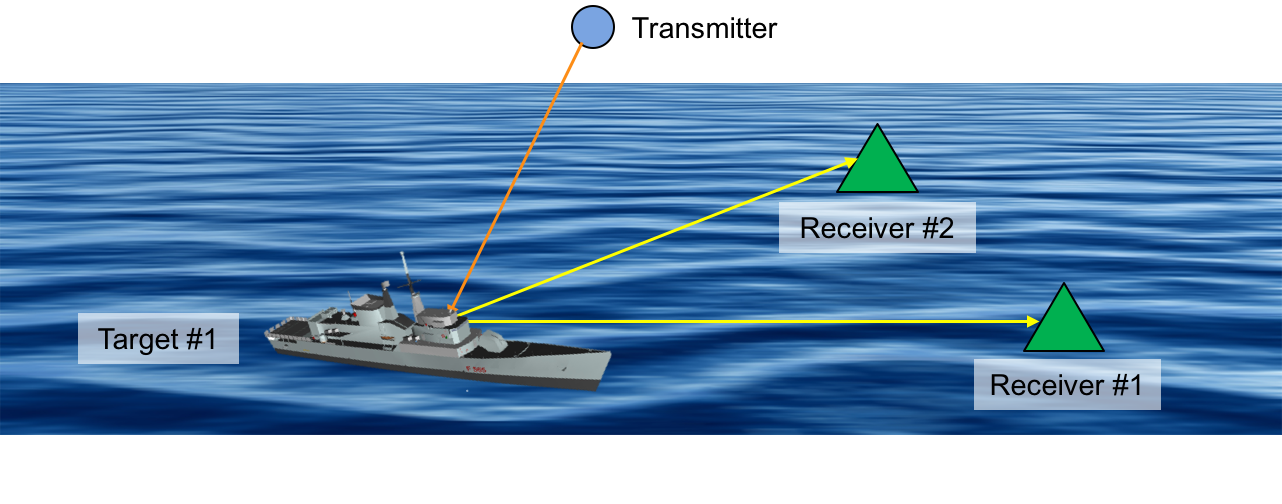
\includegraphics[width=5in]{../media/multistatic/ms_rf_concept.png}
  \end{center}
  \renewcommand{\baselinestretch}{1} \small\normalsize
  \begin{quote}
    \caption[Multistatic RF Sensor Networks Concept]{Multistatic RF Sensor Networks Concept\label{ms_fig:1}}
  \end{quote}
\end{figure}
\renewcommand{\baselinestretch}{2} \small\normalsize

\section{Beam Width}
The beam width of an antenna is defined as the angle between the half power points in the antenna pattern.

\subsection{One Way}
The one way antenna beam width, $\theta$, is simply the beam width of the forward propagating beam.

\subsection{Two Way}
The two way antenna beam width, $\theta_2$, is the beam width of the return beam that propagates in both directions. For the monostatic case, we can compute this as the one way beam width of the square of the antenna pattern. In most cases, $\theta_2 \approx \frac{1}{\sqrt{2}}\theta$.

\section{RADAR Range Equation} 
The RADAR range equation provides a deterministic method to calculate received signal levels and is the workhorse for analyzing RADAR system performance. Thi equation is the first step towards building a statistical model, as it captures the underlying physics.

\subsection{Monostatic Case}
The traditional monostatic RADAR range equation is shown in Equation \ref{intro_eq:1} and is generated by assuming spherically propagating waves and taking the product of four components: the power received at the target, the power reflected by the target, the power received back at the transmitter, and the effective area of the transmitter\cite{skolnik_handbook}.
  \begin{equation}
  \label{intro_eq:1}
 P_r = \left(\frac{P_tG_t}{4\pi R^2}\right) \left(\sigma \right)\left(\frac{1}{4\pi R^2}\right)\left( \frac{G_t\lambda^2}{4\pi} \right) = \frac{P_tG_t^2\sigma\lambda^2}{\left(4\pi\right)^3R^4}
  \end{equation}
The projected power is spread out over a sphere of radius equal to the slant range, $R$, which gives the factor of $\left( 4\pi R^2 \right)^{-1}$. The total projected power is the transmitted power, $P_t$, multiplied by the antenna gain, $G_t$. The RADAR cross section (RCS), $\sigma$, defines the amount of power intercepted and reflected. The effective area of the antenna is then $\frac{G_t\lambda^2}{4\pi}$.
  
We can divide Equation \ref{intro_eq:1} by the noise power to represent the RADAR equation in terms of signal to noise ratio (SNR) as shown in Equation \ref{intro_eq:2} \cite{skolnik_handbook}.
\begin{equation}
    \label{intro_eq:2}
\text{SNR} = \frac{P_r}{P_n} = \frac{P_tG_t^2\sigma\lambda^2}{\left(4\pi\right)^3 R^4k_BTBF_n}
\end{equation}
In this equation, $k_B$ is the Boltzmann constant, $B$ is the receiver bandwidth, $T$ is the receiver temperature and $F_n$ is the receiver noise figure. Nominally, $B$ is taken to be the inverse of the pulse width to accomodate matched filter processing and $T$ is taken to be $300$ K.

\subsection{Bistatic Case}
In the bistatic case, we need to consider each path separately as the ranges, antenna gains, and RCS are all likely different. The standard bistatic RADAR range equation is shown in Equation \ref{intro_eq:3}.
  \begin{equation}
  \label{intro_eq:3}
 P_r = \frac{P_tG_tG_r\sigma_B\lambda^2}{\left(4\pi\right)^3R_1^2R_2^2}
  \end{equation}
In this equation, $G_t$ is the antenna gain for the transmitter, $G_r$ is the antenna gain for the receiver, $\sigma_B$ is the bistatic RCS, $R_1$ is the slant range along the first path, and $R_2$ is the slant range along the second path.

The bistatic RADAR range equation in terms of SNR is shown in Equation \ref{intro_eq:4}.
\begin{equation}
    \label{intro_eq:4}
\text{SNR} = \frac{P_tG_tG_r\sigma_B\lambda^2}{\left(4\pi\right)^3 R_1^2R_2^2k_BTBF_n}
\end{equation}

\subsection{Propagation Factors}
The use of propagation factors allow us to include atmospheric effects in the RADAR range equation. These effects can include absorption from atmospheric gases and weather such as rain or snow as well as rollups for the effects of multipath reflections.

\section{Probability of Detection}

\section{Processing Gains}
\subsection{Coherent Processing}
\subsection{Noncoherent Processing}
\subsection{M of N Detection}